\chapter{Escolha dos gráficos}

Jogos estilo \textit{Kart} são conhecidos por sua jogabilidade acessível e dinâmica, que combina elementos de corrida e combate, e por seus personagens carismáticos e coloridos. No gênero temos vários estilos visuais a serem explorados, desde gráficos 2D até gráficos 3D realistas.

\section{Jogos 2D (ou 2.5D)}

O primeiro \textit{Mario Kart} foi lançado em 1992 para o Super Nintendo Entertainment System (SNES) e desde então a série se tornou uma das mais populares e bem-sucedidas da Nintendo. O jogo foi desenvolvido em 2D, principalmente por limitações técnicas da época, mas o jogo realiza uma simulação de 3D, com artes em 2D que se movem em um ambiente 3D simulado, o que é conhecido como gráficos 2.5D.

\subsection{Gráficos e lógica bidimensional}

Esse estilo de gráficos foi muito explorado na época dos consoles de 16 bits, como o SNES e o Mega Drive, e ainda é muito popular em jogos \textit{indie} e \textit{mobile}, devido à sua simplicidade e facilidade de desenvolvimento. Além disso, esse estilo de gráficos é muito charmoso e nostálgico, o que atrai muitos jogadores, por isso é uma ótima opção para jogos de Kart (\cite{graficos2.5D}). Para uma melhor compreensão, veja a Figura \ref{fig:mario-kart}.

Podemos explicar este estilo 2.5D como um jogo 2D que simula um ambiente 3D, com personagens e cenários em 2D, mas com movimentação e câmera simulando um ambiente 3D. Isso é feito através de técnicas de renderização e animação, que dão a ilusão de profundidade e movimento tridimensional.

\subsection{Implementação moderna, lógica 2D e gráficos 3D}

Hoje em dia não temos tal limitação técnica, mas o estilo 2.5D ainda é muito popular, principalmente em jogos indie e mobile, devido à sua simplicidade e facilidade de desenvolvimento. Isso facilita a produção de jogos com gráficos bonitos e charmosos, porém com uma lógica que só considera um espaço bidimensional, o que simplifica o desenvolvimento e a programação.

Um exemplo de um jogo onde se usa esse estilo de gráficos é o \textit{Mario Wonder} (\cite{marioWonder}), recente e tem toda a sua lógica programada em um espaço limitado 2D, porém sua aparência visual é completamente processada em 3D.

\begin{figure}[H]
    \centering
    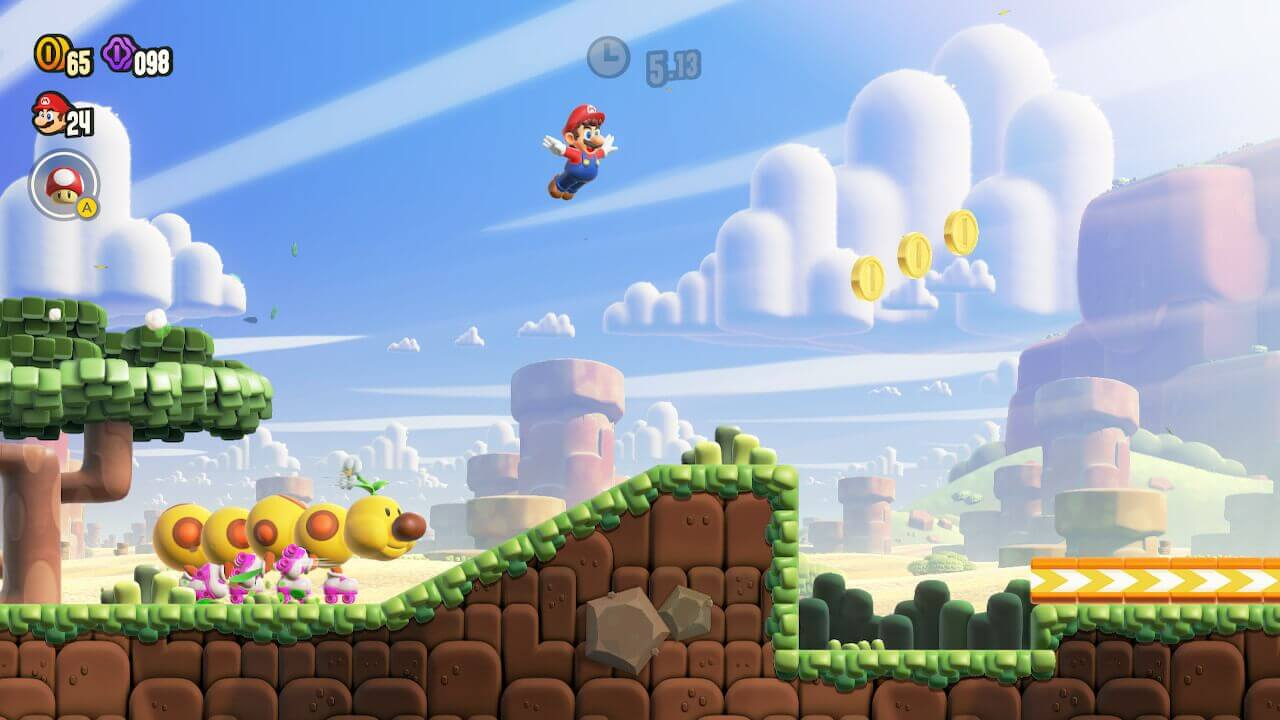
\includegraphics[width=0.8\textwidth]{figuras/Mario Wonder.jpg}
    \caption{Mario Wonder. \cite{marioWonder}}
    \label{fig:mario-wonder}
\end{figure}

\section{Jogos 3D}

Outra opção seria desenvolver o jogo totalmente em 3D, com gráficos realistas e ambientes tridimensionais, o que daria uma sensação de imersão e realismo muito maior, mas também seria muito mais complexo e demorado de desenvolver. Além disso, o estilo 3D é mais comum em jogos de corrida de Kart mais recentes, como \textit{Crash Team Racing Nitro-Fueled} e \textit{Blur}, que possuem gráficos realistas e ambientes tridimensionais, com texturas e efeitos visuais muito bem detalhados.

Para isso devemos pensar num ambiente tridimensional na totalidade, não somente quanto à parte visual, mas também com a lógica do jogo, que deve considerar um espaço tridimensional, com movimentação e colisão em três dimensões. Isso é muito mais complexo e demorado de desenvolver, mas o resultado é muito mais imersivo e realista, o que pode atrair mais jogadores e fãs do gênero.

\section{Decisão}

Optamos pelo desenvolvimento do \textit{USP Kart} em 2.5D, lógica bidimensional, mas com gráficos 3D, utilizando do OpenGL moderno para renderização e animação, o que gera uma sensação de profundidade e movimento tridimensional, mas com uma lógica simplificada e mais fácil de desenvolver. Isso viabilizou a produção do jogo, permitindo seu desenvolvimento de maneira compatível com a duração de um trabalho de conclusão de curso.